\documentclass{article}
\newcommand\myname{Paul Löhr}
\newcommand\myStuyProgramm{Studiengang Verkehrssystemmanagement}


\usepackage[ngerman]{babel}
\usepackage{geometry}
\usepackage{fancyhdr}
\usepackage{graphicx}
\usepackage{tabularx}
\usepackage{xcolor}

\fancyhf{}
\pagestyle{fancy}

\lhead{\raisebox{-1\height}{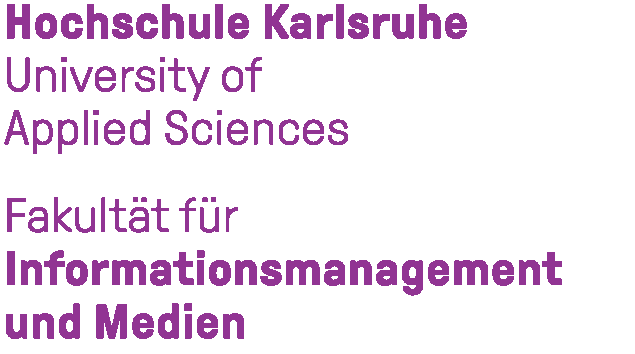
\includegraphics[width=4cm]{bilder/HKA_IMM_Wortmarke.pdf}}}
\rhead{\raisebox{-1\height}{
\includegraphics[width=4cm]{bilder/HKA_IMM.pdf}}}
\renewcommand{\headrulewidth}{0pt}
\setlength{\headheight}{100pt}


\lfoot{\textcolor{violet}{\myname}}
\cfoot{\textcolor{violet}{\myStuyProgramm}}
\renewcommand{\footrulewidth}{0pt}


\renewcommand{\arraystretch}{2}


\begin{document}

%Überschrift
\begin{center}
    {\huge \textbf{VSM-Vorlage}}
    \vspace{10pt}
\end{center}


\section*{Überschrift 1}
Wir möchten euch herzlich zur bevorstehenden Vortragsreihe "Informatik im 
Verkehrswesen" einladen, die im Rahmen der Veranstaltung "Grundlagen Informatik" 
stattfinden wird. Diese Vortragsreihe zielt darauf ab, die Verbindung zwischen der 
Informatik und dem Verkehrswesen aufzuzeigen und euch einen Einblick in die spannenden 
Anwendungen und Entwicklungen in diesem Bereich zu geben.

\subsection*{Mittwoch, 1.November 2023}

\begin{table}[h]
    \begin{tabularx}{\textwidth}{l|X}
        Zeit & Programm \\
        \hline
        6:45 Uhr & Treffpunkt HKA, Moltkestraße 30 \\
        7:00 Uhr & Abfahrt mit dem Bus nach Prag \\
        Im Bus & Zimmeraufteilung und Gruppenverkündung \\
        Ca. 15 Uhr & Ankunft in Prag und Check-in im Czech Inn \\
        Ab 16 Uhr & Möglichkeiten finden, am nächsten Morgen zum CTU Campus zu gelangen \\
        Abend & Zur freien Verfügung
    \end{tabularx}
    \end{table}

\subsection*{Überschrift 2}
In der heutigen Zeit sind Technologien und digitale Lösungen nicht mehr aus dem Verkehrsbereich
wegzudenken. Vom intelligenten Verkehrsmanagement über die Navigationssysteme bis hin zur
Fahrzeugkommunikation – die Informatik spielt eine zentrale Rolle in der Gestaltung effizienter, 
sicherer und nachhaltiger Verkehrssysteme. Wir möchten euch inspirieren und motivieren, 
die vielfältigen Möglichkeiten zu erkunden, die euch in dieser spannenden Schnittstelle zwischen 
Informatik und Verkehrswesen erwarten.


\end{document}